\documentclass[10pt]{beamer}

%\usepackage[backend=bibtex,firstinits=true,style=verbose-inote,citestyle=authortitle]{biblatex}
\usepackage{bm}
\usepackage{graphicx}
\usepackage{subcaption}
\usepackage{amsmath}
\usepackage{amsfonts}
\usepackage{makecell}
\usepackage{filecontents}
\usepackage{biblatex}
\newcommand{\expect}[2][]{
\ifthenelse{\equal{#1}{}}{
\mathbb{E}\left[#2\right]
}{
\underset{#1}{\mathbb{E}}\left[#2\right]
}}

\newcommand{\cov}[2][]{
\ifthenelse{\equal{#1}{}}{
\text{Cov}\left[#2\right]
}{
\underset{#1}{\text{Cov}}\left[#2\right]
}}


\newcommand{\var}[2][]{
\ifthenelse{\equal{#1}{}}{
\text{Var}[#2]
}{
\underset{#1}{\text{Var}}[#2]
}}

\newcommand{\loss}[2][]{
\ifthenelse{\equal{#1}{}}{
\mathcal{L}(#2)
}{
\mathcal{L}_{#1}(#2)
}}

\newcommand{\kl}[2]{
\text{D}_\text{KL}[#1 \parallel #2]
}

\newcommand{\R}{\mathbb{R}}
%\newcommand{\Prob}{\mathbb{P}}

\newcommand{\1}[1]{\mathds{1}\{#1\}}


%\usecolortheme{dolphin}
\setbeamertemplate{navigation symbols}{}
\setbeamertemplate{section in toc}{\inserttocsectionnumber.~\inserttocsection}

\addbibresource{references.bib}


\title{Meta Generation}
%\subtitle{}
\author{Ivan Skorokhodov}
%\date{}
%\logo{
\includegraphics[height=1cm]{images/ipavlov-logo.png}}

\newcommand{\citepaper}[1]{\citetitle{#1} by \citeauthor{#1}}

%\graphicspath{{./images}}

%\usetheme{lucid}
\begin{document}

\begin{frame}
    \titlepage
\end{frame}


\begin{frame}{Implicit Neural Representations}
\begin{itemize}
    \item\pause INR is a neural network $f_\varphi(x,y)$ which takes coordinates $(x,y)$ and produces a pixel value:
    \begin{figure}
        \centering
        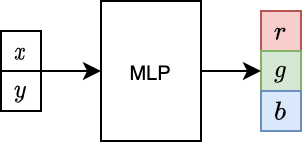
\includegraphics[width=0.3\textwidth]{images/inr}
    \end{figure}
    \item\pause We can generate the whole image by computing the value of $f_\varphi(x,y)$ at each coordinate
    \item\pause I.e. we have \textit{1 image} = \textit{1 INR}
\end{itemize}
\end{frame}


\begin{frame}{Benefits of INRs}
    \begin{itemize}
        \item\pause They carry more ``complete'' information about a signal:
        \begin{itemize}
            \item Usual 2D arrays of pixels are discretized version of a signal
            \item INRs are continuous and carry information ``between'' the pixels
            \item This allows one to have ``superresolution out-of-the-box''
        \end{itemize}
        \item\pause They are popular in 3D deep learning since they are cheaper to generate and operate with than 3D objects
    \end{itemize}
\end{frame}


%\begin{frame}{Problems with INRs}
%\begin{itemize}
%    \item\pause INRs are not that small:
%    \begin{itemize}
%        \item\pause SIREN/FFN use $\approx 256\times 5$ MLPs with 3000 epochs
%        \item\pause But fitting low-frequency images is much easier\footnote{a note to myself: show face/knot examples here}
%    \end{itemize}
%    \item\pause It requires to train an INR on an image to obtain the INR and each training procedure (currently) takes a lot of time (up to 10 minutes).
%    \item\pause Community does not have a good understanding of how to work with them
%\end{itemize}
%\end{frame}


%\begin{frame}{Transposed convolutions are problematic}
%\begin{itemize}
%    \item\pause They lack the biological plausibility of normal convolutions
%    \item\pause They produce artefacts (like checkerboard patterns)
%    \item\pause You have to change architecture for each output size
%    \begin{itemize}
%        \item\pause This can be solved by interpolation procedures to some extent, but for tasks like segmentation this would lead to coarse predictions
%    \end{itemize}
%    \item\pause They struggle to capture scene geometry:
%    \begin{itemize}
%        \item\pause For example, it's hard to draw long straight lines (so generated walls ``wobble'', circles are curved, etc)
%        \item\pause CoordConv paper showed that it cannot learn to classify a pixel given its coordinates
%    \end{itemize}
%\end{itemize}
%\end{frame}



\begin{frame}{INR-GAN}
Train a generator to produce INRs
    \begin{figure}
        \centering
        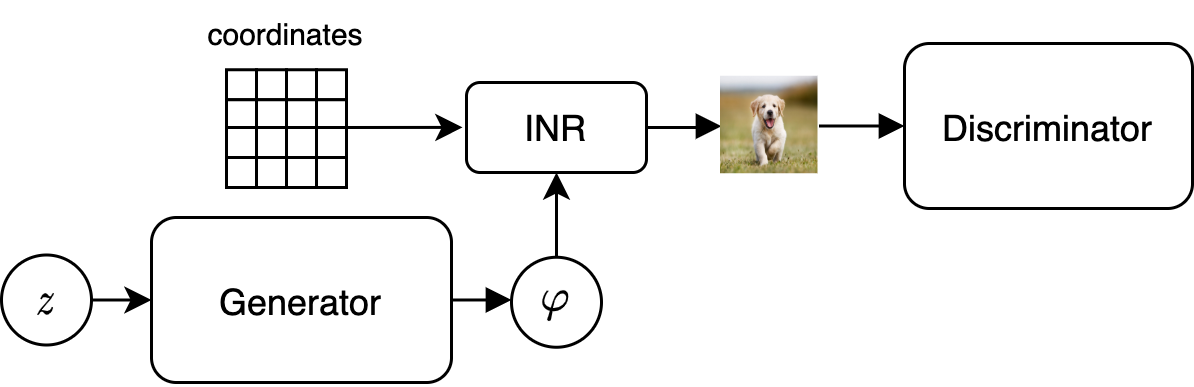
\includegraphics[width=0.9\textwidth]{images/inr-gan}
    \end{figure}
%    \item\pause Discriminator can operate:
%    \begin{itemize}
%        \item\pause on top of images
%        \item\pause on top of INRs (but this would require converting the whole dataset into INRs)
%    \end{itemize}
\end{frame}


\begin{frame}{Advantages compared to traditional GANs}
\begin{itemize}
    \pause\item A unified generator architecture for images/audio/video/3D-shapes
    \pause\item Better biological plausibility
    \pause\item We can generate different resolutions for different parts of an image
    \begin{itemize}
        \pause\item Imagine that we generate an image of a human on a sky background
        \pause\item We can use dense set of coordinates for a human and a sparse set of coordinates for the sky
        \pause\item It is good since it is impossible to do so for a normal GAN
    \end{itemize}
    \pause\item We can generate spherical images (and images on any surface)
    \pause\item We can use ``random resolutions'' loss to train a high-resolution GAN
    \pause\item We can train our generator on images of extreme resolution by using a ``super-resolution'' loss:
    \begin{itemize}
        \pause\item Train an INR-GAN normally on, for example, $256\times256$ images
        \pause\item Additionally, compute random dense patches and make the discriminator to distinguish between real/fake dense patches
        \pause\item (Provide global context if needed)
    \end{itemize}
    \item\pause It should be cheaper to use for some domains (audio, 3D, video, extreme-resolution images)
    \item\pause Progressive growing is easier to incorporate
\end{itemize}
\end{frame}


\begin{frame}{Samples on LSUN bedroom 64x64 (FID: 12.75)}
\begin{figure}
    \centering
    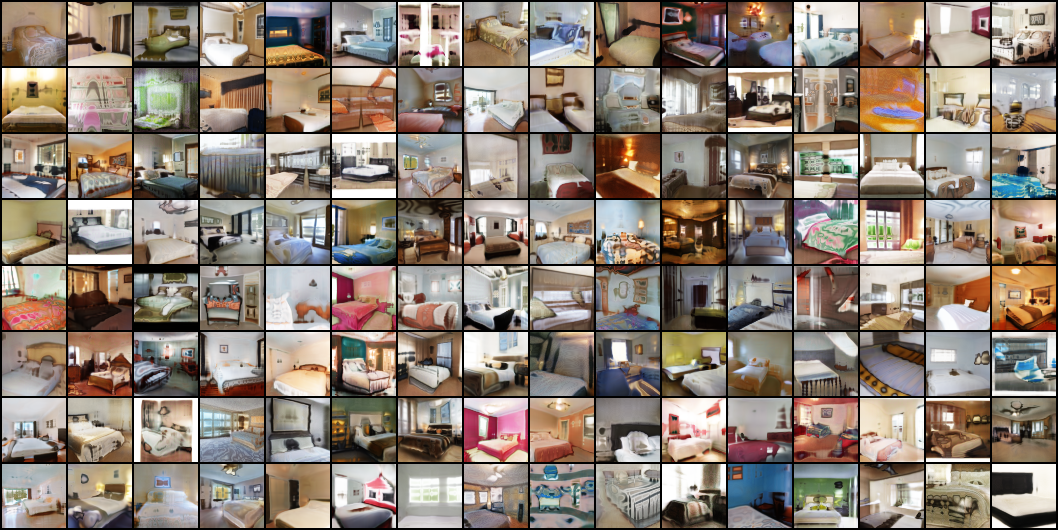
\includegraphics[width=\textwidth]{images/samples}
\end{figure}
\end{frame}

%\begin{frame}{Interpolations on LSUN bedroom 64x64}
%\begin{figure}
%    \centering
%    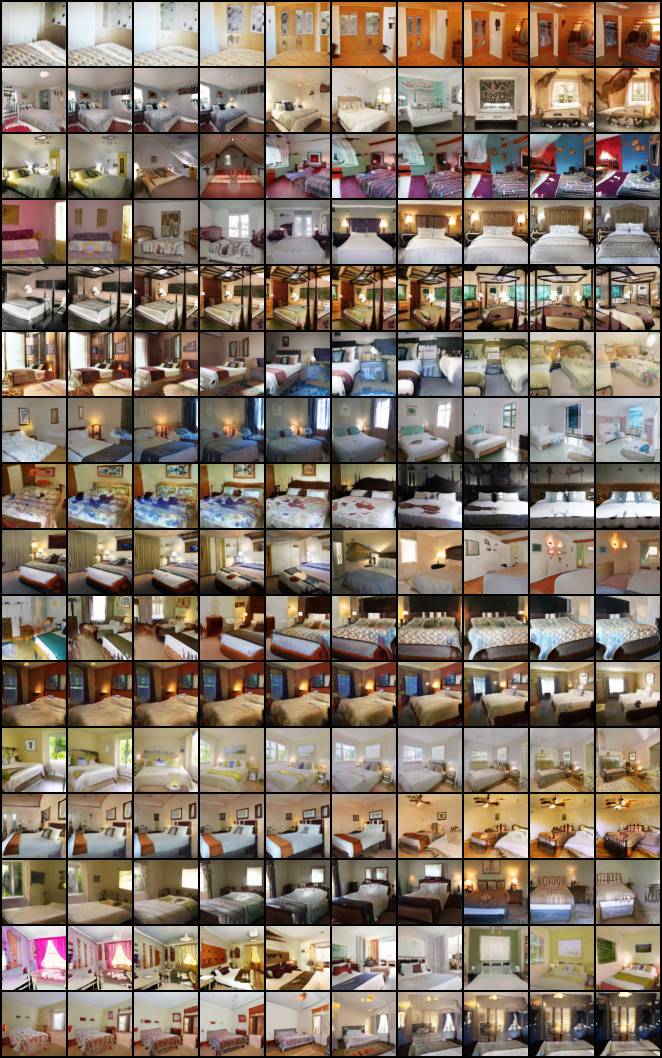
\includegraphics[width=\textwidth]{images/interpolations}
%\end{figure}
%\end{frame}
%
%\begin{frame}{Activations histograms in the INR}
%\begin{figure}
%    \centering
%    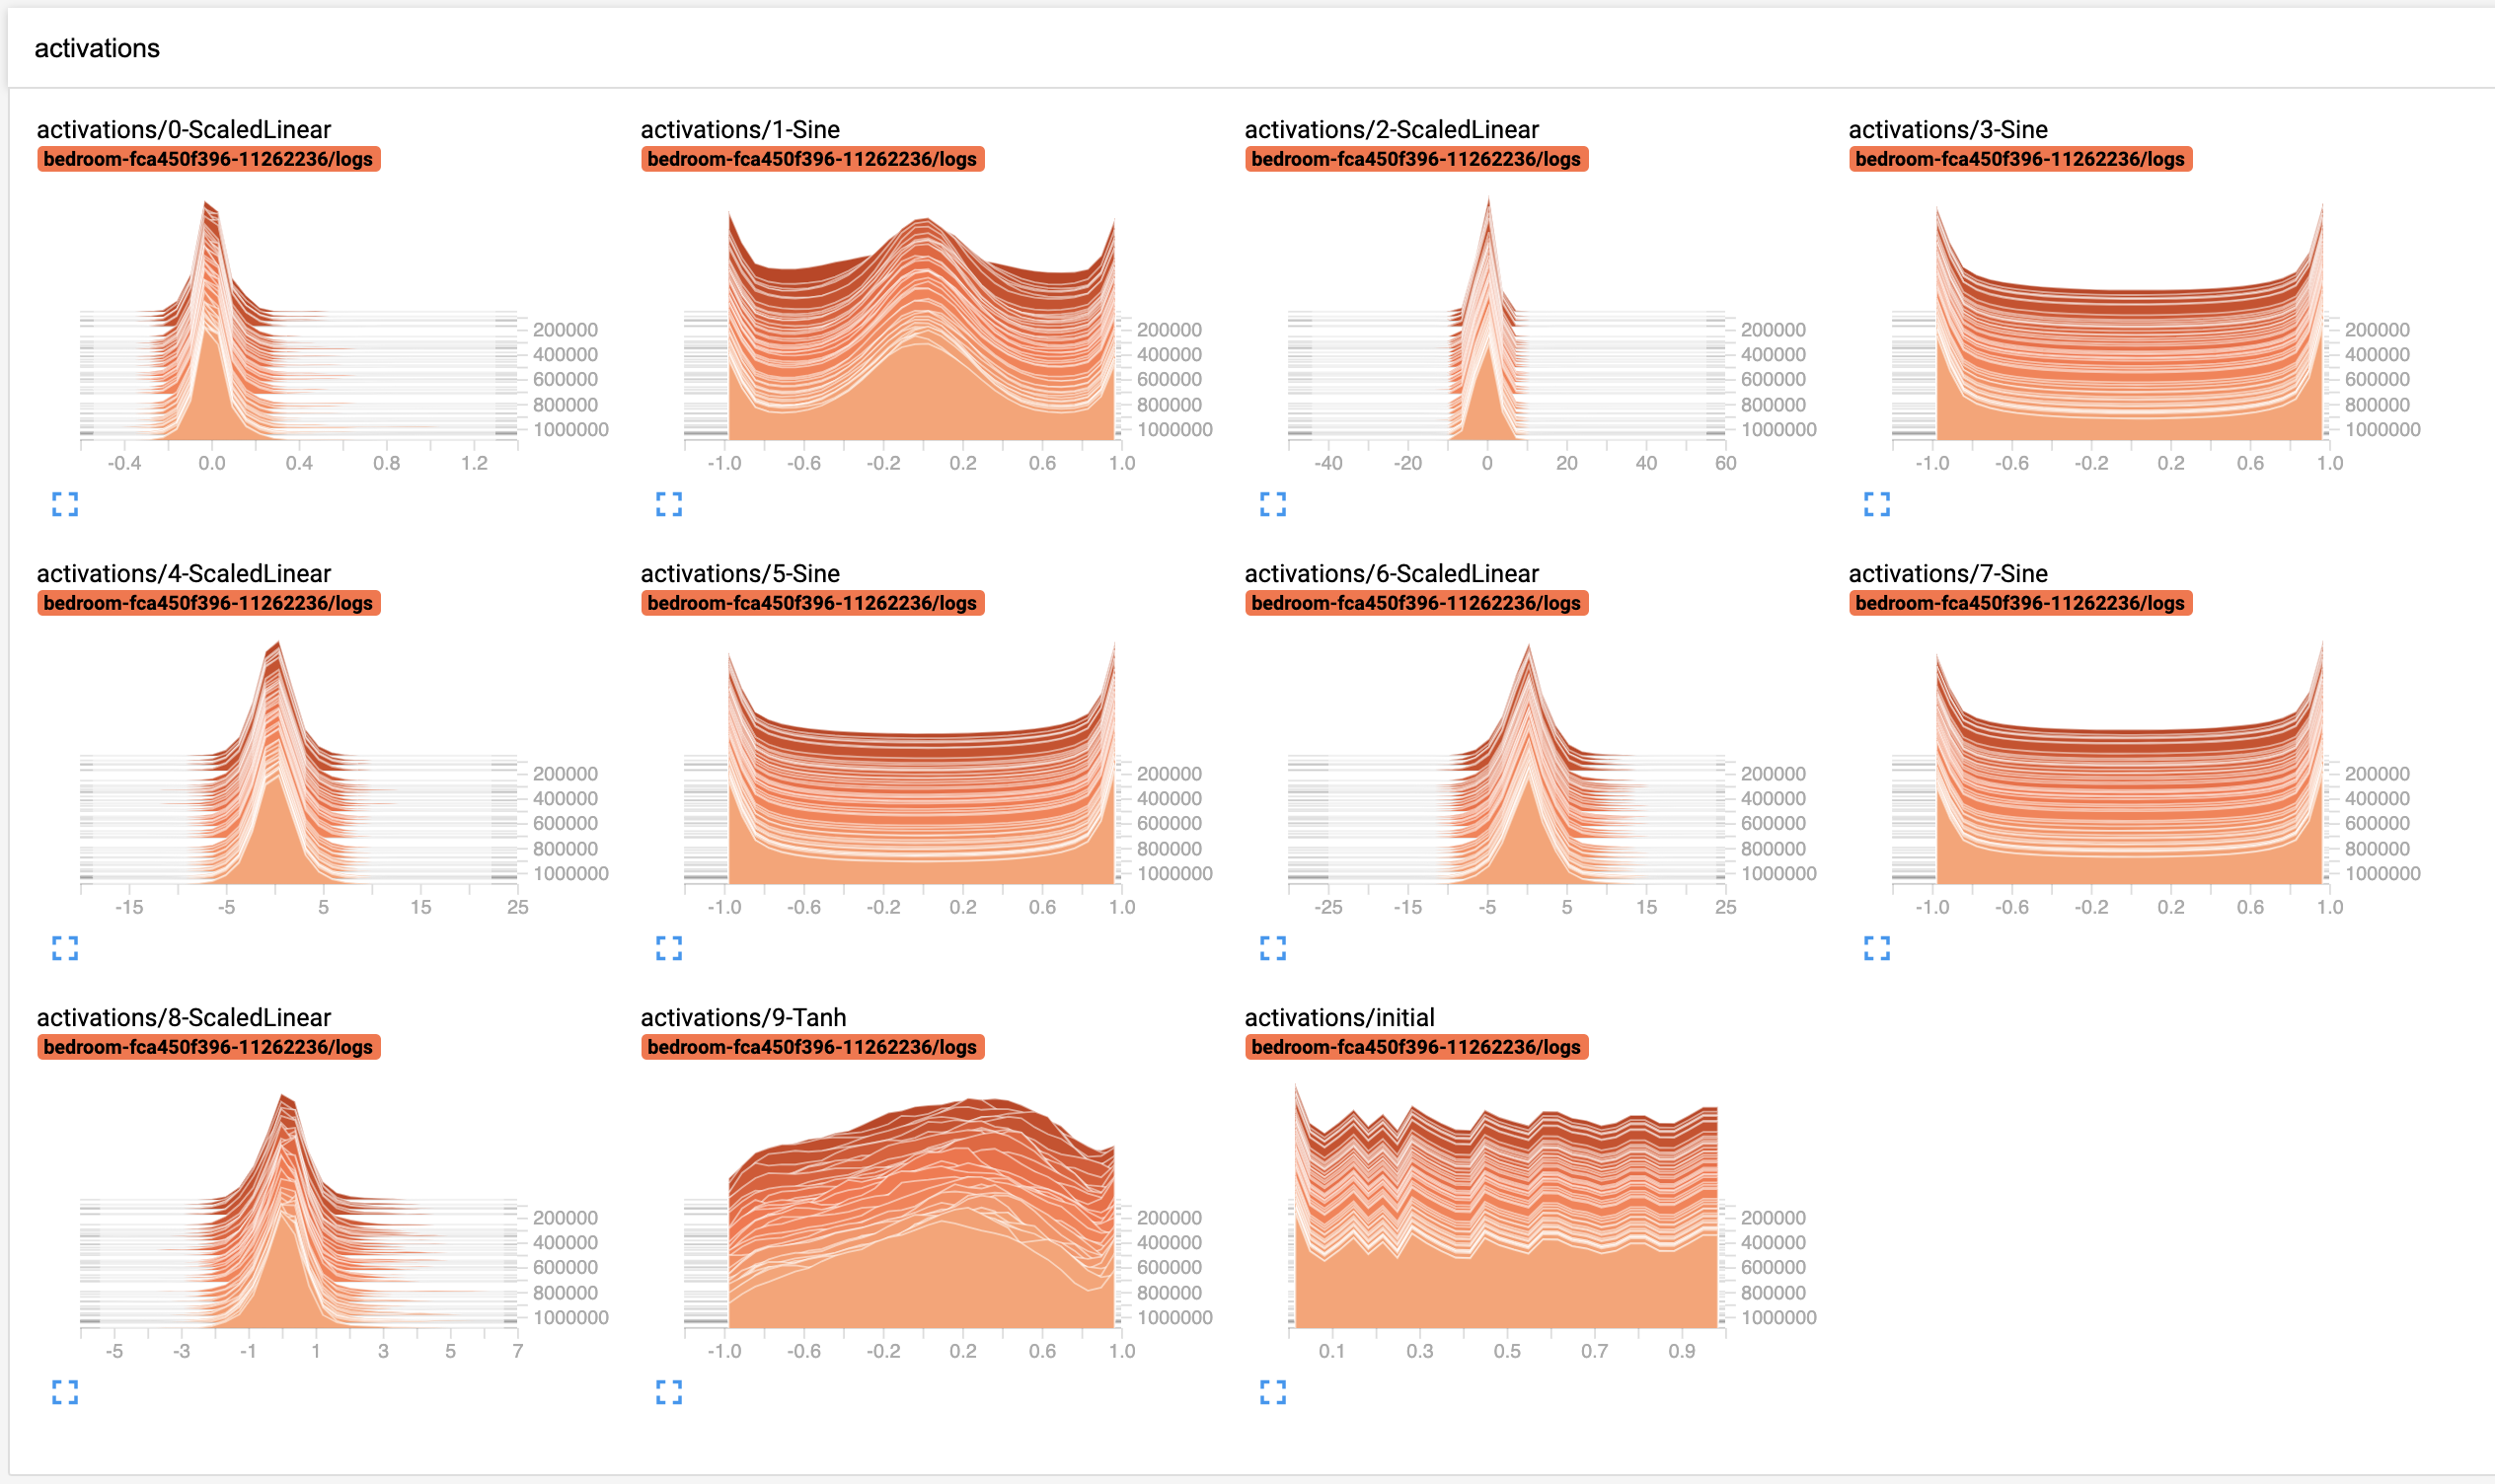
\includegraphics[width=\textwidth]{images/activations}
%\end{figure}
%\end{frame}

\begin{frame}{Q: FourierINR vs SIREN}
\pause
SIREN:
\begin{itemize}
    \item\pause Use $\sin(x)$ activation function everywhere
    \item\pause Initialize the weights with $\sigma = \sqrt{2/n_\text{in}}$
    \item\pause For the first layer, use $\sigma_1 = \sigma / 30$ and multiply the activations by 30 afterwards. Why? Do we suffer from small gradients when we use $\sin(x)$?
\end{itemize}

\pause 
Fourier INR:
\begin{itemize}
    \item\pause Use $\sin(x)$ and $\cos(x)$ for the first layer (and concat them together)
    \item\pause Use traditional layers and activations on top of that
    \item\pause Initialize the first layer with $\sigma \sim 100$.
\end{itemize}

Which one do you like more?
\end{frame}


%\begin{frame}{``GAN stability'' paper baseline}
%\begin{itemize}
%    \item\pause Use ``GAN-stability'' model as a baseline
%    \item\pause 
%\end{itemize}
%\end{frame}


\begin{frame}{Size/quality tradeoff for INR architecture}
\begin{table}[]
\begin{tabular}{|l|c|c|}
\hline
Type & MAE (50 imgs) & \#params \\ \hline
Linear & 0.047 & $n^2 + n$ \\
SELinear & 0.050 & $n^2 + n$ \\
mFiLM & 0.914 & $3n$ \\
mFiLM -norm & 0.656 & $3n$ \\
mFiLM -norm +scale & 0.089 & $3n$ \\
Factorized ($r=10$) & 0.285 & $2nr + n$ \\
FactorizedSE ($r=10$) & 0.059 & $2nr + n$ \\
AdaIN & 0.089 & $2n$ \\ \hline
\end{tabular}
\end{table}
\textit{All of them ran in 3.6 iters/sec} on 1080 Ti and used ~10 GB GPU memory\footnote{Except for AdaIN, which took more memory for some reason.}.
\end{frame}


\begin{frame}{Changes overview}
Implementing some tricks increased FID from $\approx$150 to 58 at 20k iterations on LSUN conference room\footnote{I didn't test each change individually}:
\begin{itemize}
    \item\pause SIREN $\to$ FourierINR
    \item\pause Generator EMA (had to remove BatchNorm)
    \item\pause WGAN-GP $\to$ R1
    \item\pause D5:G1 $\to$ D1:G1 ticks
    \item\pause batch size 32 $\to$ batch size 64 
    \item\pause LRs 0.002/0.0002 $\to$ 0.0001/0.0002 for G/D (like in StyleGAN)\footnote{What LR should we use for G? Is it equivalent to the mapping network?}
    \item\pause INR size $64 \times 5 \to 256 \times 5$
    \item\pause INRLinear $\to$ INRFactorizedSELinear
    \item\pause WGAN loss $\to$ NS loss (results are in progress)
    \item\pause Residual weight $0.0 \to 0.1$
\end{itemize}
\end{frame}


\begin{frame}{Model samples for LSUN bedroom 128x128}
\begin{figure}
    \centering
    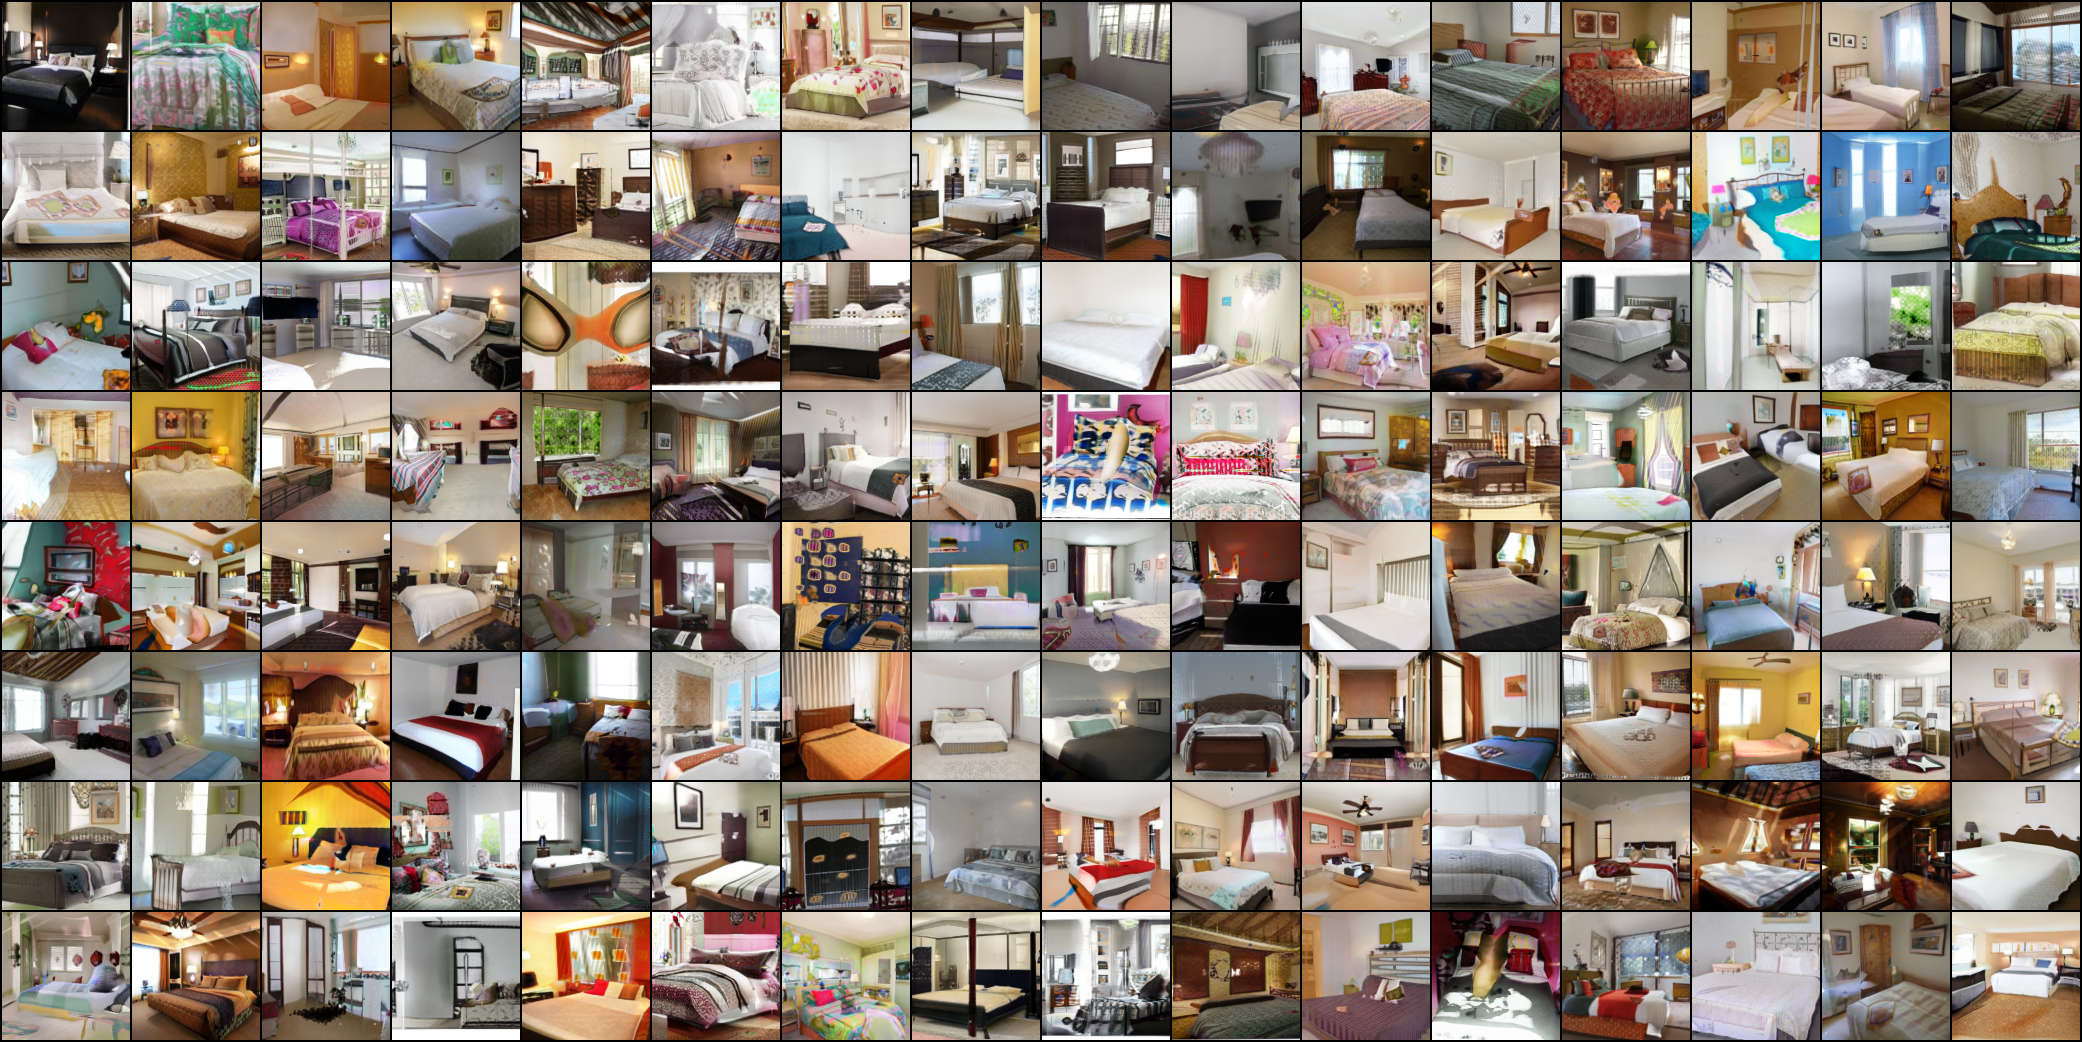
\includegraphics[width=\textwidth]{images/best-model-samples-august-30}
    \caption{Model samples for LSUN bedroom 128x128 after 500k iterations. FID is 7.2}
\end{figure}    
\end{frame}


\begin{frame}{Bluntly increasing the model size}
Bluntly increasing the model size does not work:
\begin{itemize}
    \item\pause For INR, increasing the size from $256 \times 5 \to 256 \times 10$ resulted in FID degradation: $12 \to 15$ FID after 40k iters
    \item\pause For G, switching from $1024 \times 5$ to:
    \begin{itemize}
        \item\pause $2048 \times 3$ backbone
        \item\pause 7 independent heads of $1024 \times 3$
    \end{itemize}
    resulted in FID degradation: $12 \to 35$ after 50k iters
    \item\pause For D, increasing the size from 10M parameters to 30M parameters didn't change FID
\end{itemize}
\end{frame}


\begin{frame}{INR natural upsampling vs bilinear upsampling}
Consider the following setup:
\begin{itemize}
    \item\pause Train an INR-GAN on $128\times 128$ images
    \item\pause Upsample to $256 \times 256$ with bilinear upsampling
    \item\pause Upsample to $256 \times 256$ with INR ``natural'' upsampling (i.e. just use a denser coordinate grid as an INR input)
\end{itemize}

\pause
Result:
\begin{itemize}
    \item\pause FID for INR natural upsampling is $\sim 2$ times better than for the bilinear upsampling:
    \begin{itemize}
        \item\pause 22 vs 41.4 after 70k iterations on LSUN bedroom
    \end{itemize}
    \item\pause But it is $\sim 2$ times worse than model's FID score on $128\times 128$ images
    \begin{itemize}
        \item\pause 22 vs 10.7 after 70k iterations on LSUN bedroom
    \end{itemize}
\end{itemize}

How to improve INR natural upsampling?
\end{frame}


\begin{frame}{Clipping G output}
\pause
\begin{itemize}
    \item\pause Instead of $w = G(z)$ compute INR weights with:
    $$w = \text{clip}(G(z), -2, 2)$$
    \item\pause This is approximately $\pm 2\sigma$ for $\mathcal{N}(0,1)$. 
\end{itemize}

\pause This does not change FID much ($8 \to 7.6$ after 300k iters on LSUN bedroom), but makes interpolations awful:
\begin{figure}
\centering
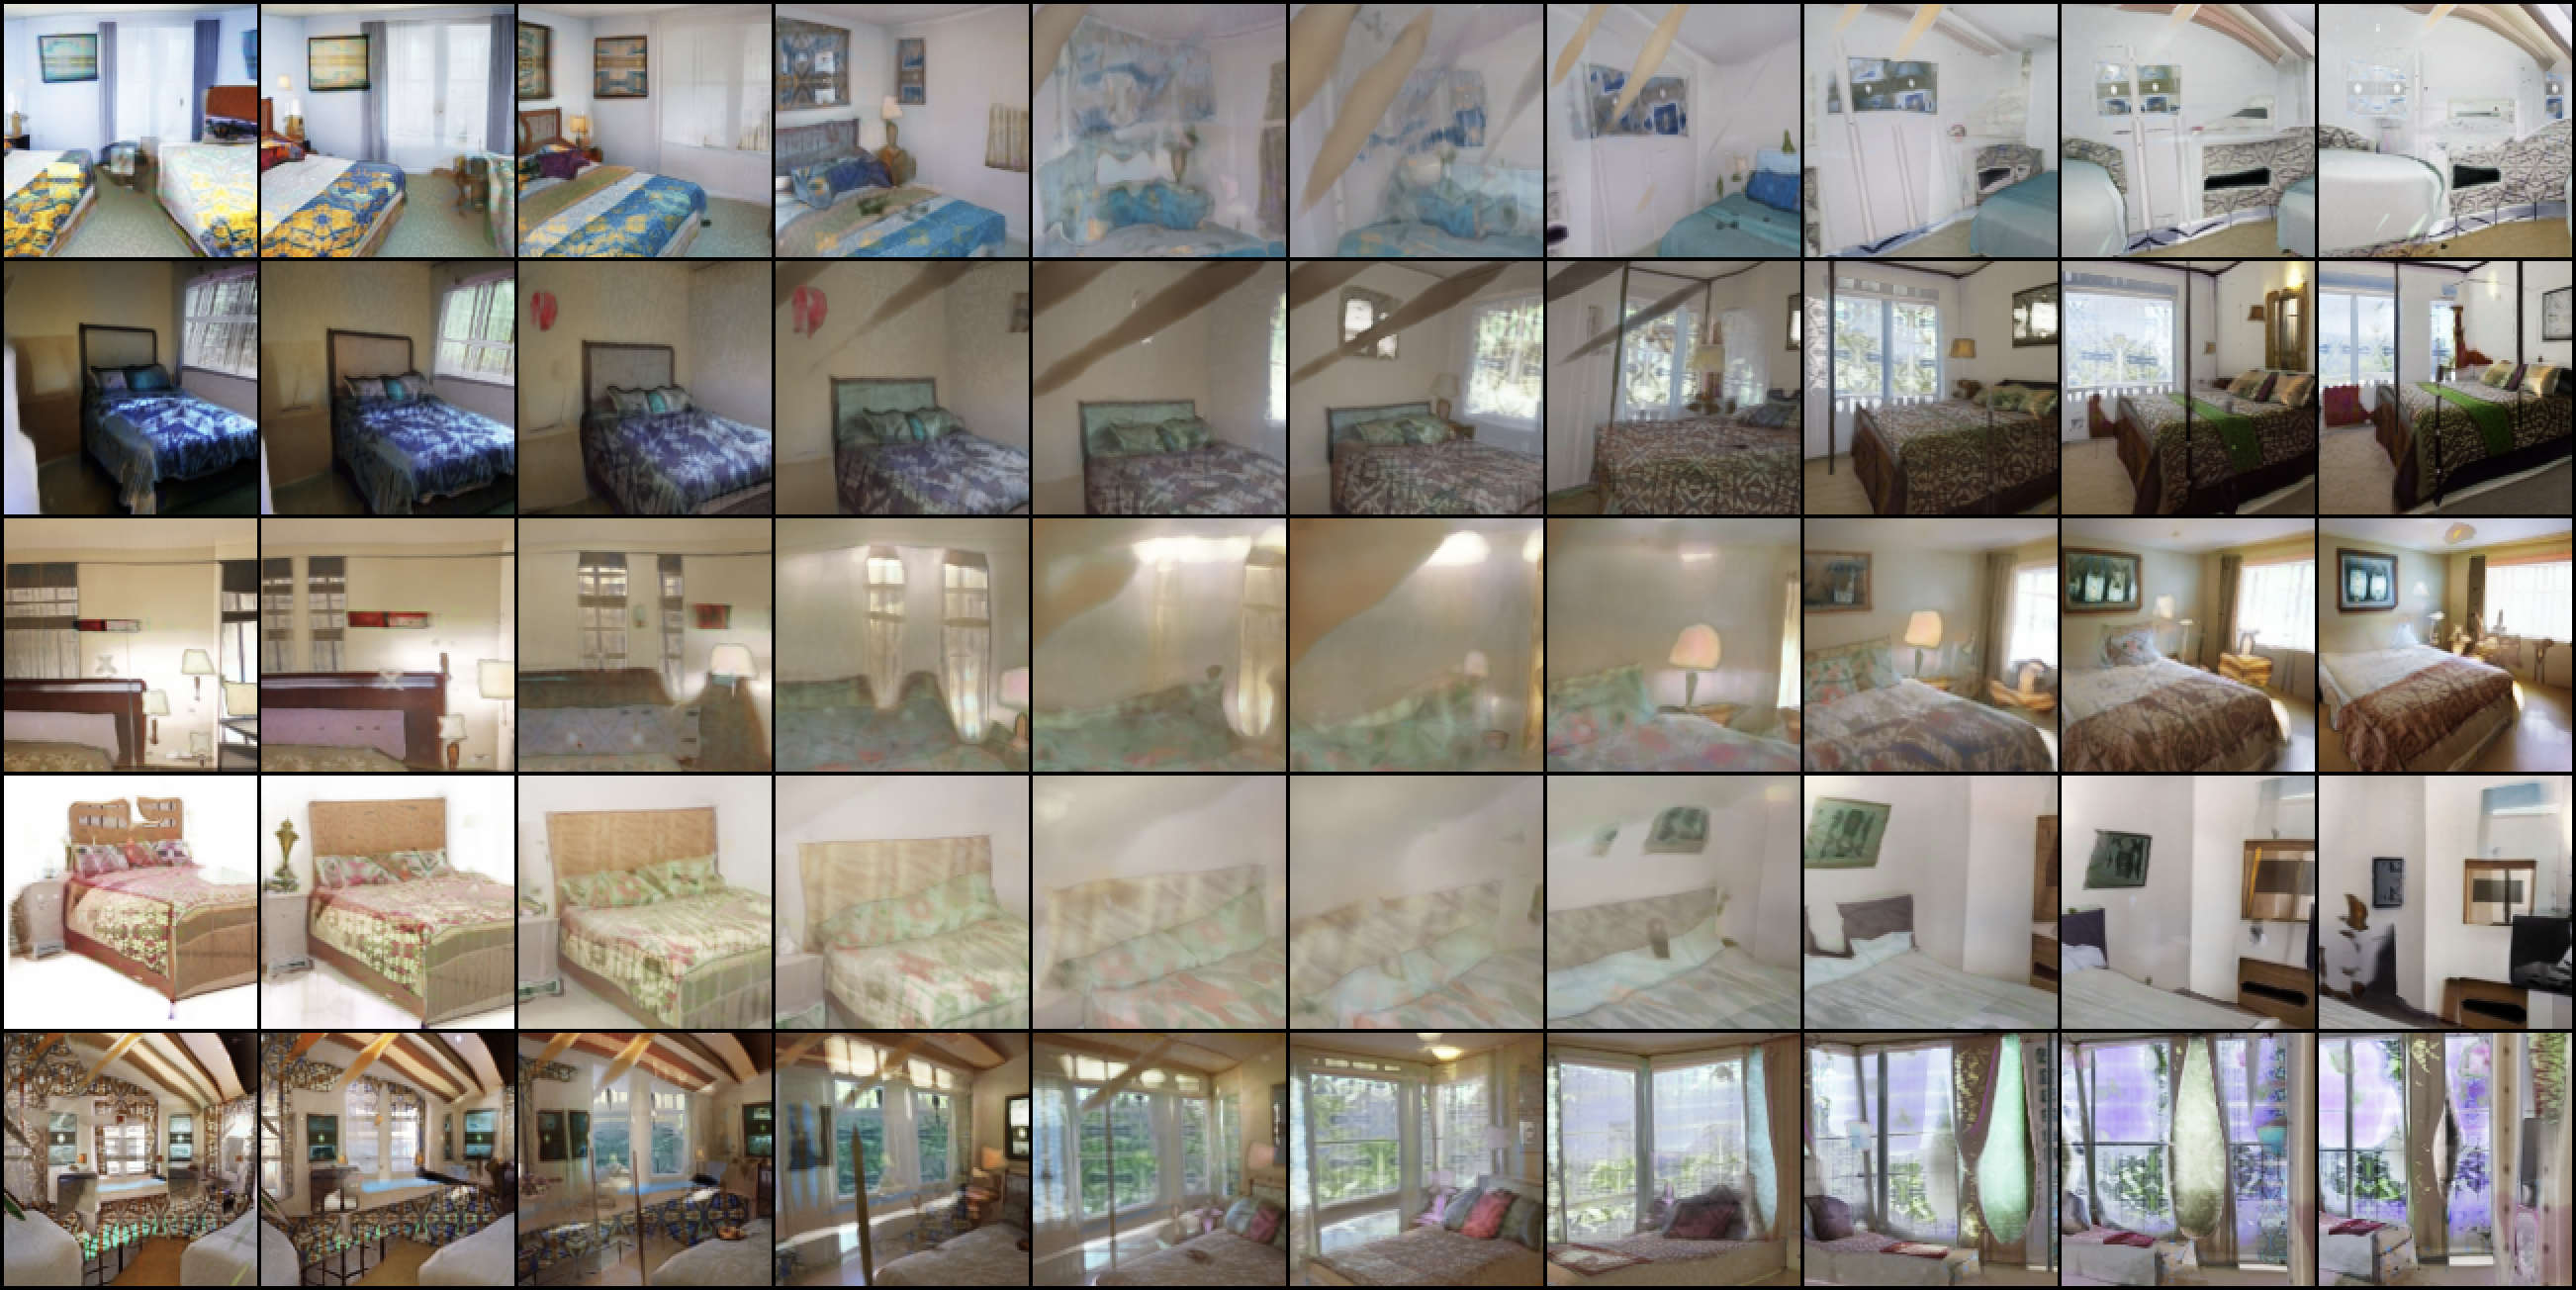
\includegraphics[width=0.7\textwidth]{images/normal_clip_lerp.png}
\end{figure}
\end{frame}


\begin{frame}{Concatenating a local patch to an image}
\begin{figure}
\centering
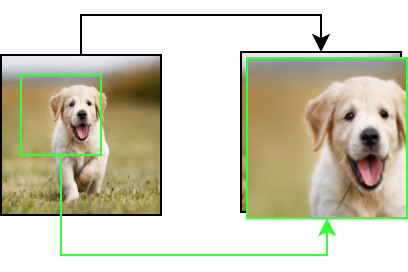
\includegraphics[width=0.7\textwidth]{images/patch-concatenation}
\end{figure}

Main idea:
\begin{enumerate}
    \item select a random image patch
    \item upsample it
    \item concatenate to the image
    \item train in such a manner
\end{enumerate}

This should force G to learn how to upsample to high-res.
\end{frame}

\begin{frame}{Concatenating a local patch to an image didn't work}
\pause

But it didn't work (LSUN bedroom $128 \times 128$):
\begin{itemize}
    \item For patch of ratio of 0.25, FID is 33
    \item For patch of ratio of 0.5, FID is 120
    \item For patch of ratio of 0.75, FID is 10.5
\end{itemize}

\pause
However, concatenating a 0.25 patch makes the gap between FID and upsampled FID lower:
\begin{itemize}
    \item FID gap is 5 while usually it is $>10$.
\end{itemize}

\pause
\textit{Q: Why did the training diverge?}
\end{frame}


\begin{frame}{Is G too weak?}
I tried to run 3 generator versions:
\begin{itemize}
    \item With 2 hidden layers
    \item With 3 hidden layers
    \item With 6 hidden layers (default option)
\end{itemize}

And they worked almost the same!
FIDs are 7.9, 7.8 and 7.65 after 350k iters on LSUN bedroom $128 \times 128$.

\textit{Q: How to check if G is too weak?}
\end{frame}


\begin{frame}{Linear generator}
\begin{figure}
\centering
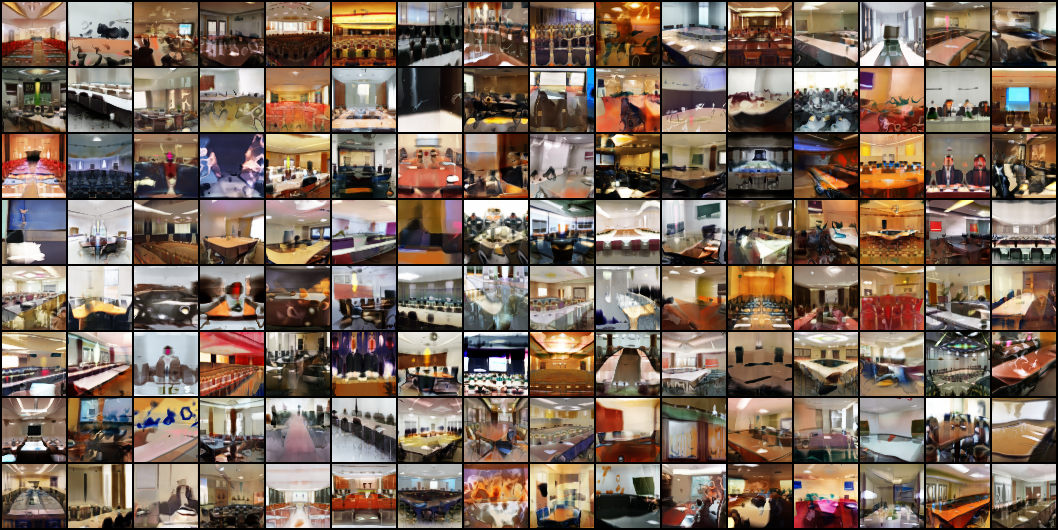
\includegraphics[width=\textwidth]{images/linear-generator}
\end{figure}
\end{frame}


\begin{frame}{Traditional INR parametrization}
\pause
Traditional INR parametrization requires $N_\varphi \times $ size matrix for G output layer.
\begin{figure}
\centering
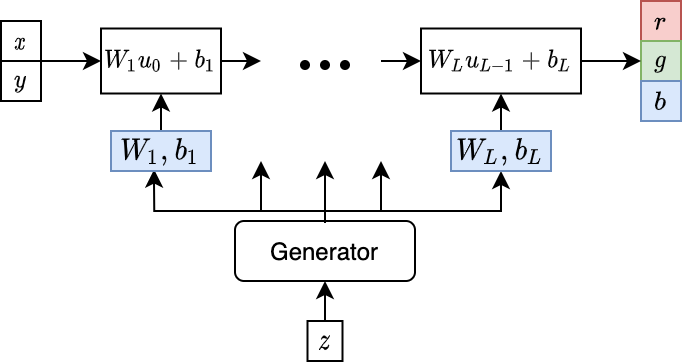
\includegraphics[width=0.7\textwidth]{images/linear-inr}
\end{figure}

\pause
That's why a good chunk of research was devoted to finding cheap but expressive INR parametrization.
\end{frame}


\begin{frame}{Factorized squeeze-and-excitation INR parametrization}
\begin{figure}
\centering
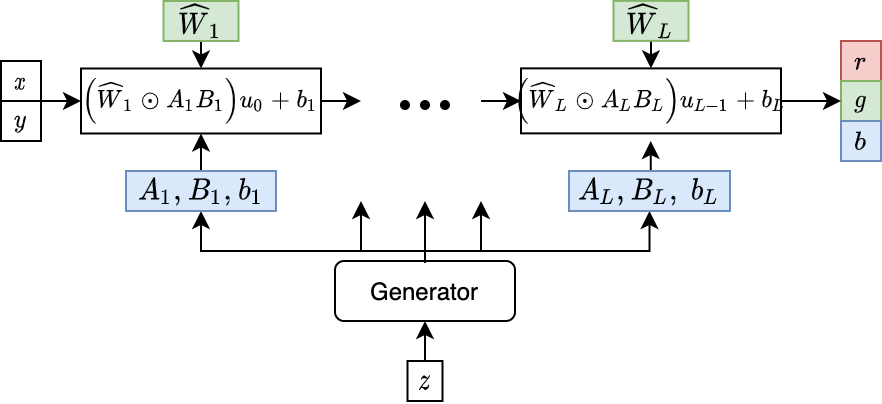
\includegraphics[width=0.7\textwidth]{images/factorized-se-linear}
\end{figure}

Idea:
\begin{enumerate}
    \item\pause For layer $\ell$, produce matrices $A_\ell, B_\ell$ of sizes $n\times r$ and $r \times n$ respectively.
    \item\pause Multiply them together to get a low-rank $\tilde{W}_\ell = A_\ell B_\ell$ of rank $r$
    \item\pause Compute $W_\ell = \hat{W}_\ell \odot \tilde{W}_\ell$ where $\hat{W}_\ell$ is a full-rank matrix shared for all images.
    \item\pause In this way, G neuromodulates existing $\tilde{W}_\ell$ and we control cost/expressivity with rank $r$.
    \item\pause In practice, $r=5$ works fine.
\end{enumerate}
\end{frame}


\begin{frame}{Going further: Multi-Modal INRs}
Idea:
\begin{itemize}
    \item\pause Let's keep not a single $\hat{W}_\ell$, but $M$ such matrices: $\hat{W}^{(1)}, \hat{W}^{(M)}$
    \item\pause Each $\hat{W}_\ell^{(m)}$ corresponds to a different mode.
    \item\pause G additionally produces a softmax distribution $p_1, ..., p_M$ and selects over different modes.
    \item\pause A good thing is that it does not increase computation burden much.
    \item\pause For reconstruction task, it worked like a charm: $0.059 \to 0.037$ for $M=100$.
    \item\pause For generation task, it performed worse: $10.5 \to 11.2$ after 200k iters on FFHQ $128 \times 128$.
\end{itemize}

\textit{Q: why didn't it work better?}
\end{frame}



\begin{frame}{Deciding upon the contributions}
What we are going to sell:
\begin{itemize}
    \item\pause Best known scores for a GAN with G consisting entirely from fully-connected layers
    \item\pause Can we say that our G has just 2 hidden layers?
    \item\pause We investigated different INR parametrizations and proposed novel FactorizedSE paramtrization
    \item\pause We show that INR interpolates much better than bilinear/nearest/cubic interpolations
    \item\pause We investigated scaling inside the INR
    \item\pause We should argue that INRs has good potential and will replace conv-based decoders someday (but leave these claims for future work):
    \begin{itemize}
        \item\pause an ability to train the model on extreme-scale images ($4096 \times 4096$)
        \item\pause out-of-the-box interpolation
        \item\pause universal G architecture for any domain (images, video, audio, etc)
    \end{itemize}
\end{itemize}

Overall, we pushed INR-GANs for image domain quite far.
Our work democratizes INR-GANs.

\textit{Q: in what form should we present what we've done?}
\end{frame}


\begin{frame}{Next step: hierarchical INR}
    I didn't think that we'll get that far. That's why this slide is empty.
\end{frame}


\begin{frame}{Next steps}
\begin{itemize}
    \item\pause Main bottleneck in INR is the hidden dimensionality which is very expensive to scale
    \item\pause Training on variable-sized images
    \begin{itemize}
        \item\pause We hope that traditional convolutions would have problems producing different-ratio images
    \end{itemize}
\end{itemize}
\end{frame}

\end{document}
